\documentclass{beamer}

\usetheme{Warsaw}
\usecolortheme[RGB={100,0,100}]{structure}
\setbeamercolor{alerted text}{fg = blue}

\usepackage[utf8]{inputenc}
\usepackage{default}
%code
\usepackage{listings}

\title{Let's play with Python and OpenCV}
\author{Omar Trinidad Gutiérrez Méndez}
\institute{División Académica de Informática y Sistemas\\ Universidad Juárez Autónoma de Tabasco}
\date{July 6, 2012}

\begin{document}

  \lstset{ %
    language=Python,                % choose the language of the code
    stringstyle=\ttfamily,
    basicstyle=\footnotesize\ttfamily,
    numbers=left,
    keywordstyle=\color{blue}, %chose the color of "words"
    frame=shadowbox,rulesepcolor=\color{black},
    showstringspaces=false,
    stepnumber=1,                 % the step between two line-numbers. If it's 1 each line will be numbered
    backgroundcolor=\color{white}   % choose the background color. You must add \usepackage{color}
  }

\begin{frame}{}
  \transdissolve
    \titlepage

%  \begin{figure}
%    \centering
%     \includegraphics[width = 2cm, height = 2.5cm]{./logoDAIS.png}
%  \end{figure}
\end{frame}

\section{Introduction}
\subsection{Computer Vision}
\begin{frame}{Computer Vision}
\transdissolve
  \pause
  \begin{block}{}
   A picture is worth a thousand words.
  \end{block}

  \pause
  \begin{itemize}[<+-| alert@+ >]
    \item The computer vision is the science and engineering
	  discipline concerned with making inferences about 
          the external world.
    \item What is an image? Is an array. An array of pixels.
    \item The goal of the computer vision is to achieve
	  something similar to the human perception.
  \end{itemize}
\end{frame}

\begin{frame}{Computer Vision}
\transdissolve
  \pause
  \begin{figure}
    \centering
     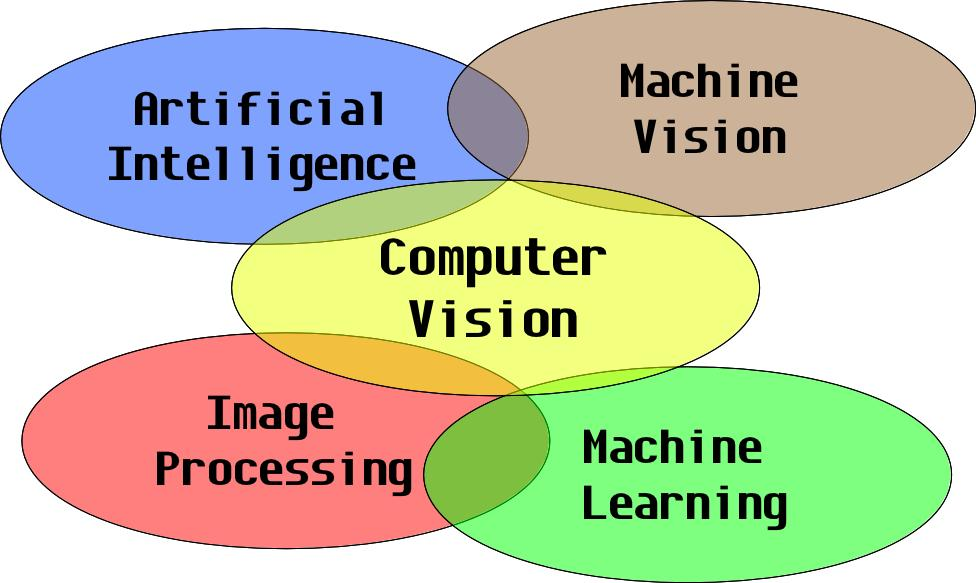
\includegraphics[width = 10cm, height = 7cm]{areas.jpg}
  \end{figure}
\end{frame}

\subsection{OpenCV}
\begin{frame}{OpenCV}
\transdissolve
  \pause
  \begin{itemize}[<+-| alert@+ >]
    \item OpenCV (Open Source Computer Vision) is a library of programming functions for real time computer vision.
    \item Is realeased under a BSD license.
    \item Languages:
      \begin{itemize}
	\item C
	\item C++
	\item Java
	\item Python ;)
      \end{itemize}
    \item Operating systems:
      \begin{itemize}
	\item Windows
	\item Mac
	\item Linux
	\item Android and iOS
      \end{itemize}
  \end{itemize}
\end{frame}

\begin{frame}{OpenCV main versions}
\transdissolve
  \pause
  \begin{itemize}[<+-| alert@+ >]
    \item Version 1.0
    \item Version 2.X.X
    \item Version 3.X.X
  \end{itemize}
\end{frame}

\begin{frame}{Binding cv versus cv2}
\transdissolve
  \pause
  \begin{itemize}[<+-| alert@+ >]
    \item Binding \texttt{cv}
       \begin{itemize}[<+-| alert@+ >]
        \item Is based in ANSI C
	\item Is tricky
	\item Uses IPLImage objects like images
       \end{itemize}
    \item Binding \texttt{cv2}
       \begin{itemize}[<+-| alert@+ >]
        \item Is based in C++
	\item Is more friendly ;)
	\item Is fastest
	\item Uses NumPy like images
       \end{itemize}
  \end{itemize}
\end{frame}

\subsection{Basic funtions}
\begin{frame}{Basic functions}
\transdissolve
  \pause
  \begin{itemize}[<+-| alert@+ >]
    \item \texttt{cv2.imread(path) -> retval}
    \item \texttt{cv2.namedWindow(name) -> None}
    \item \texttt{cv2.destroyWindow(name) -> None}
    \item \texttt{cv2.imshow(title, image)}
    \item \texttt{cv2.imwrite(path, image)}
    \item \texttt{cv2.waitKey(time)}
    \item \texttt{cv2.startWindowThread()}
  \end{itemize}
\end{frame}

{\setbeamertemplate{background canvas}{
  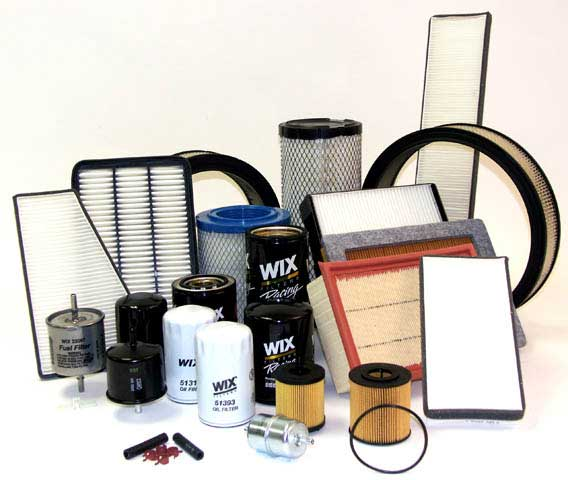
\includegraphics[width=\paperwidth, height=\paperheight]{filters.jpg}
}
\begin{frame}{Basic filters}
 
\end{frame}
}

\begin{frame}{Some basic filters}
\transdissolve
  \pause
  \begin{itemize}[<+-| alert@+ >]
    \item \texttt{cv2.blur(image, kernel) -> image}
    \item \texttt{cv2.Laplacian(image, depth) -> image}
    \item \texttt{cv2.cvtColor(image, code*) -> image}
    \item \texttt{cv2.threshold(image, threshold, maxval, type*) -> image}
    \item \texttt{cv2.dilate(image, kernel) -> image}
    \item \texttt{cv2.erode(image, kernel) -> image}
    \item \texttt{cv2.getStructuringElement(shape*, size) -> structure}
  \end{itemize}
\end{frame}

\section{Examples}
\subsection{Simple camera}
\begin{frame}[fragile]
  \frametitle{A very simple camera}
    \transdissolve
  \pause
\begin{lstlisting}[language = Python]
import cv2
cam = cv2.VideoCapture(0)
while True:
  img = cam.read()[1]
  cv2.imshow("Window", img)
  if cv2.waitKey(5) == 32:
    break
\end{lstlisting}
\end{frame}

\subsection{Object detection}
\begin{frame}[fragile]
  \frametitle{An example with FITS files}
    \transdissolve
    \pause
\begin{itemize}
  \item We will play with stars ;)
  \begin{itemize}
   \item The first step is load a FITS file.
   \item Apply \texttt{cvtColor} and \texttt{threshold} functions to the image.
   \item Use \texttt{floodFill} function to coloring the stars.
   \item Draw rectangles in the objects.
   \item Slow? \pause Ha', very slow.
  \end{itemize}
\end{itemize}
\end{frame}

\begin{frame}[fragile]
  \frametitle{Good idea and bad idea}
    \transdissolve
  \pause
\begin{itemize}
 \item Bad idea: Traverse all the items in an array.
\begin{lstlisting}[language = Python]
for x in xrange(height):
  for y in xrange(width):
    image.itemset(x, y, 0, data.item(x,y))
\end{lstlisting}
  \item Worst idea: Use indexing syntax.
\begin{lstlisting}[language = Python]
for x in xrange(height):
  for y in xrange(width):
    image[x, y] = data[x,y]
\end{lstlisting}
  \item Good ideas:
    \begin{itemize}
     \item If you feel the need for speed, go for built-in functions. \textit{Guido Van Rossum}.
     \item Read \texttt{An Optimization Anecdote} in \url{http://www.python.org/doc/essays/list2str/}
    \end{itemize}
\end{itemize}
\end{frame}

\subsection{Tracking color}
\begin{frame}[fragile]
  \frametitle{Searching the yellow color}
    \transdissolve
    \pause
  \begin{itemize}
   \item Use the simple camera and apply the blur filter.
   \item Convert the image to HSV color model and get a kind of threshold (color detection).
   \item Get the moments of the image
   \item Draw anything
  \end{itemize}
\end{frame}

\section{Conclusions}
\begin{frame}{OpenCV today}
  \begin{itemize}[<+-| alert@+ >]
    \item OpenCV 2.4.2 has been released (two days ago)
    \item Support for CUDA NVIDIA
    \item Support for Android
    \item Support for iOS
    \item Each version of OpenCV Python wrapper is more \textit{pythonic}
  \end{itemize}
\end{frame}

\section{References}
\begin{frame}{References}
  \begin{itemize}[<+-| alert@+ >]
    \item Computer Vision Class by Jitendra Malik.
    \item OpenCV
    \item A Tool for Hand-Sign Recognition by Rios Soria.
  \end{itemize}
\end{frame}

\begin{frame}{Thanks!}
  \begin{block}{About me}
   @omar\_trinidad \\
   \url{omar.vpa@gmail.com}
  \end{block}
  \begin{figure}
    \centering
     
\includegraphics[width = 2cm, height = 2.5cm]{./omar_simpson_version.jpg}
  \end{figure}
  \begin{block}{}
   Questions?
  \end{block}

\end{frame}
\end{document}
